
\documentclass[11pt]{article}
\usepackage[margin=0.78in]{geometry}
\usepackage{booktabs}
\usepackage{array}
\usepackage{graphicx}
\usepackage{float}
\usepackage{amsmath}
\usepackage{hyperref}
\hypersetup{colorlinks=true, linkcolor=blue, urlcolor=blue}
\setlength{\parskip}{0.45em}
\setlength{\parindent}{0pt}
\renewcommand{\arraystretch}{1.12}

\title{Rolling LightGBM ML Report\\\large Five-Action TP2 Strategy Selection}
\author{ML-Based Trading of TP2-Inspired Violations in SPY American Call Options}
\date{June 22, 2026}

\begin{document}
\maketitle

\section{Purpose}

This report is the first leakage-safe ML pass. The model chooses among five actions at the first
conservative TP2 violation date:

\[
\text{skip},\quad \text{trade T1},\quad \text{trade T2},\quad \text{trade K1},\quad \text{trade K2}.
\]

Labels use the first-liquid exit policy. Features are restricted to signal-date values and
lifecycle aggregates from event days \(\le 0\). Future reversion dates, exit dates, realized
P\&L, and future lifecycle rows are excluded from features. The LightGBM decision is per episode:
for each test violation it may choose skip, T1, T2, K1, or K2.

\section{Dataset}

\begin{center}
\begin{tabular}{lr}
\toprule
Quantity & Value \\
\midrule
Episode rows & 226,577 \\
Usable feature columns & 132 \\
Primary 2017-forward rows & 173,123 \\
Early robustness rows & 53,454 \\
Skip labels & 167,067 \\
T1 labels & 20,013 \\
T2 labels & 21,593 \\
K1 labels & 10,224 \\
K2 labels & 7,680 \\
\bottomrule
\end{tabular}
\end{center}

The removed all-null optional features are:
feature\_A\_gamma, feature\_A\_rho, feature\_B\_gamma, feature\_B\_rho, feature\_C\_gamma, feature\_C\_rho, feature\_D\_gamma, feature\_D\_rho.

\section{Rolling Design}

Primary folds use three training years, one validation year for threshold tuning, and one untouched
test year. The primary evaluation begins at 2017 because 2013 is partial and 2014--2016 have much
smaller conservative episode counts.

\section{Results}

\begin{center}
\resizebox{\linewidth}{!}{%
\begin{tabular}{rrrrrrrlrrr}
\toprule
Year & Rows & Selected & Executed & Invalid & Hit rate & ML P\&L & Threshold & Action-label acc. & Balanced action acc. \\
\midrule
2021 & 20,588 & 392 & 384 & 8 & 23.2\% & -\$1.18M & 0.800 & 77.8\% & 21.6\% \\
2022 & 6,604 & 1,077 & 979 & 98 & 43.3\% & -\$10.1K & 0.475 & 68.9\% & 28.9\% \\
2023 & 12,731 & 763 & 435 & 328 & 62.3\% & \$778.2K & 0.050 & 88.3\% & 28.7\% \\
2024 & 34,167 & 5,134 & 2,912 & 2,222 & 61.7\% & \$2.15M & 0.325 & 80.1\% & 33.0\% \\
2025 & 41,577 & 3,542 & 2,373 & 1,169 & 62.0\% & \$183.9K & 0.050 & 80.3\% & 28.7\% \\
2026 & 9,335 & 3,966 & 1,589 & 2,377 & 19.7\% & \$70.7K & 0.275 & 58.5\% & 32.4\% \\
\bottomrule
\end{tabular}
}
\end{center}

Aggregate LightGBM test P\&L across all primary test years is \$1.99M.
Every reported decision is made per episode. The report intentionally excludes fixed-strategy
hindsight comparisons so the results cannot be confused with a different decision problem.


\begin{figure}[H]
  \centering
  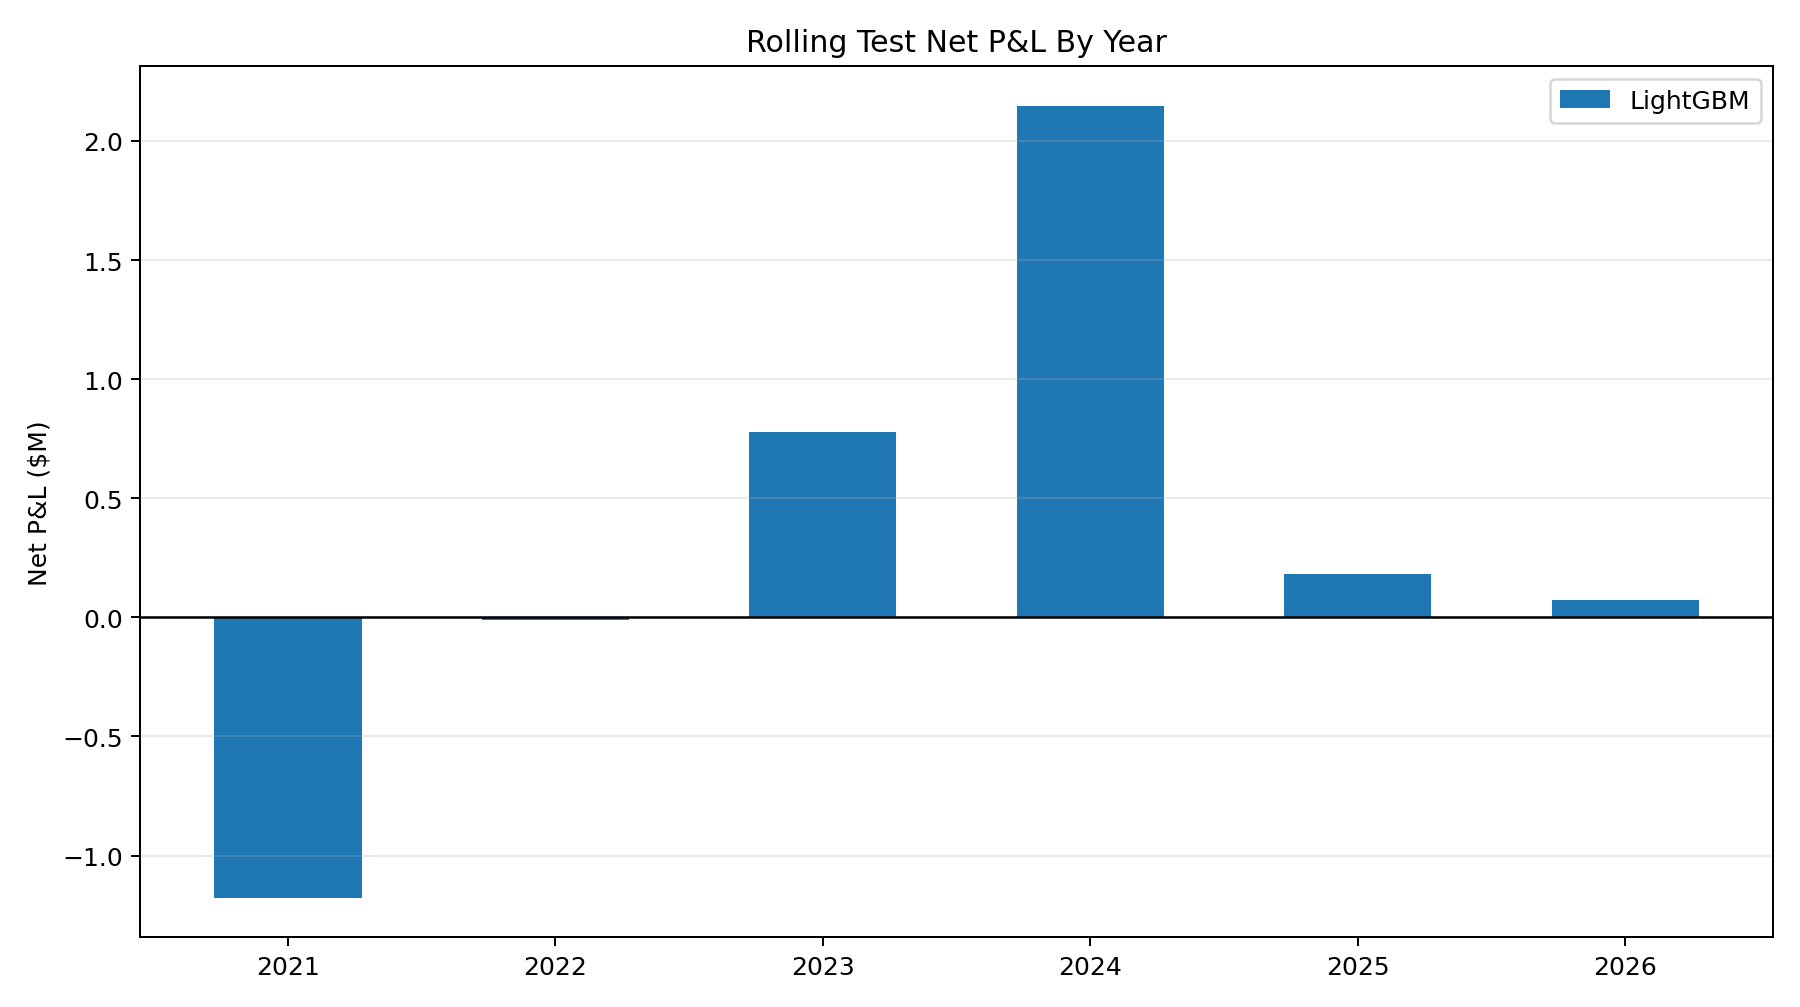
\includegraphics[width=0.92\linewidth]{figures/ml_lightgbm_yearly_pnl.png}
  \caption{Rolling test P\&L by year for the per-episode LightGBM five-action policy.}
  \label{fig:ml-yearly-pnl}
\end{figure}



\begin{figure}[H]
  \centering
  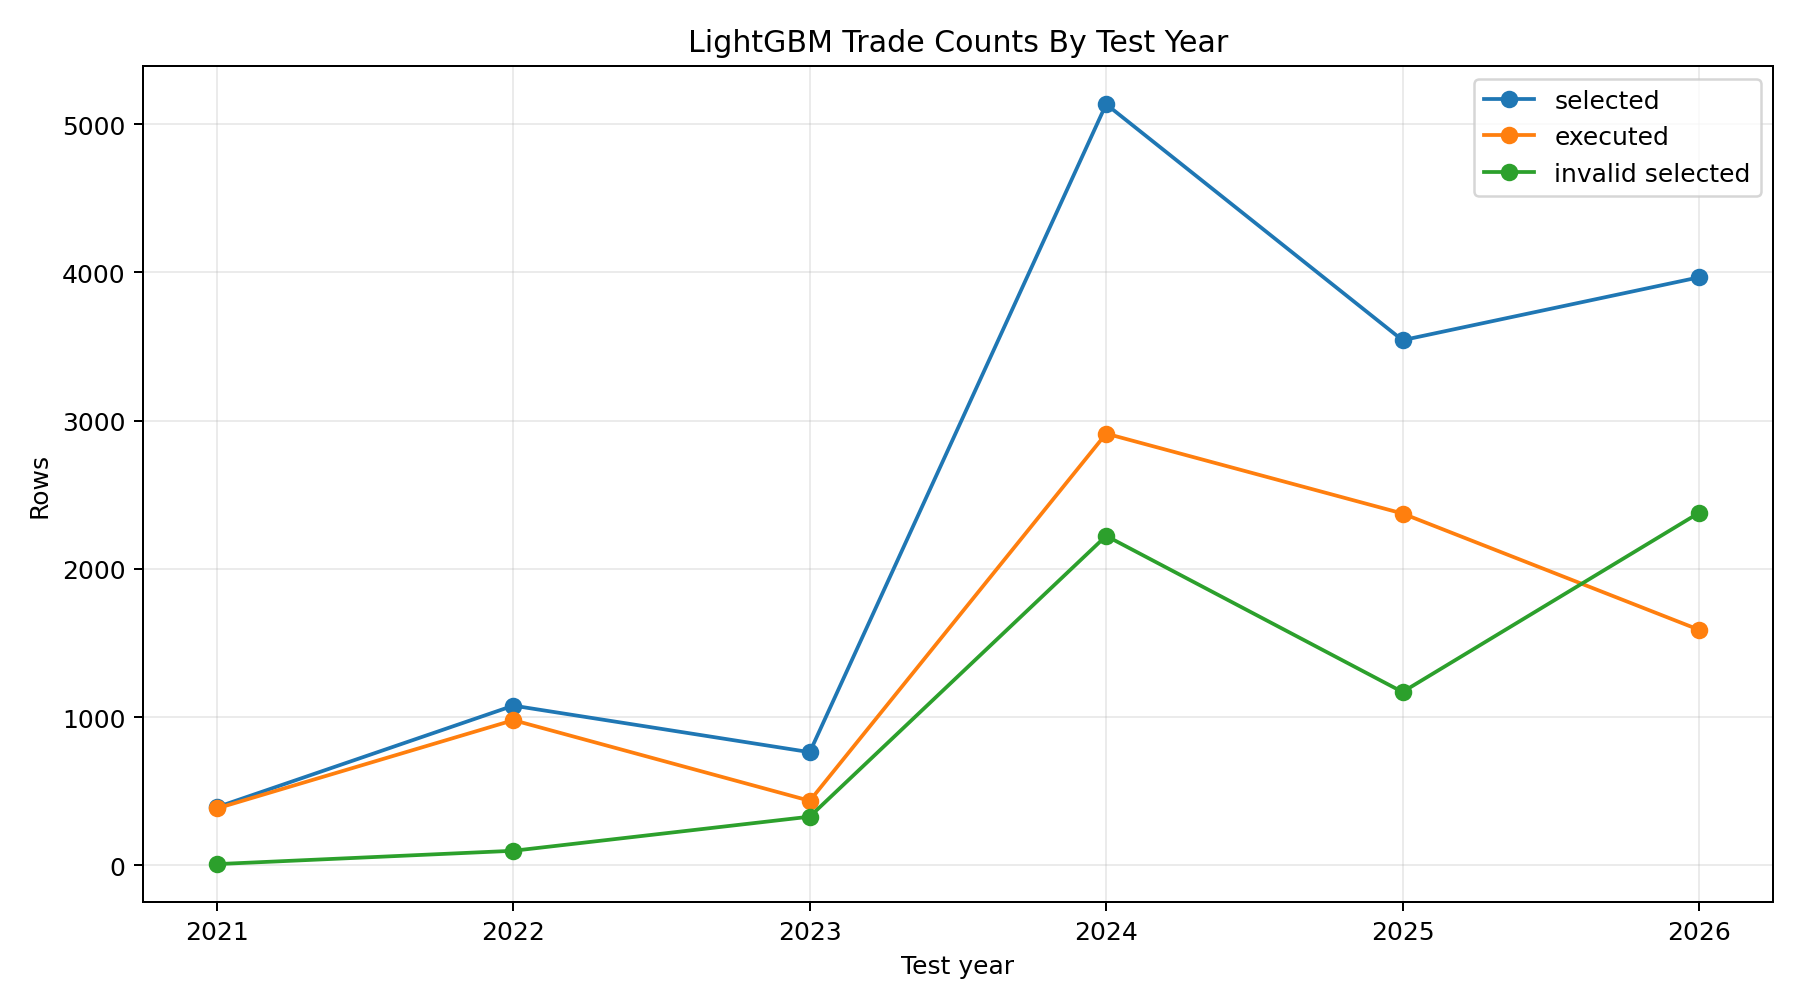
\includegraphics[width=0.92\linewidth]{figures/ml_lightgbm_trade_counts.png}
  \caption{Selected, executed, and invalid selected rows by test year.}
  \label{fig:ml-trade-counts}
\end{figure}


\section{Action Usage}

The next table shows the exact action chosen by the model in each test year. These counts are
per episode, not one strategy per year.

\begin{center}
\begin{tabular}{rrrrrr}
\toprule
Year & Skip & T1 & T2 & K1 & K2 \\
\midrule
2021 & 20,196 & 85 & 25 & 12 & 270 \\
2022 & 5,527 & 70 & 295 & 645 & 67 \\
2023 & 11,968 & 61 & 450 & 218 & 34 \\
2024 & 29,033 & 578 & 3,001 & 1,551 & 4 \\
2025 & 38,035 & 204 & 1,258 & 696 & 1,384 \\
2026 & 5,369 & 0 & 3,787 & 175 & 4 \\
\bottomrule
\end{tabular}
\end{center}


\begin{figure}[H]
  \centering
  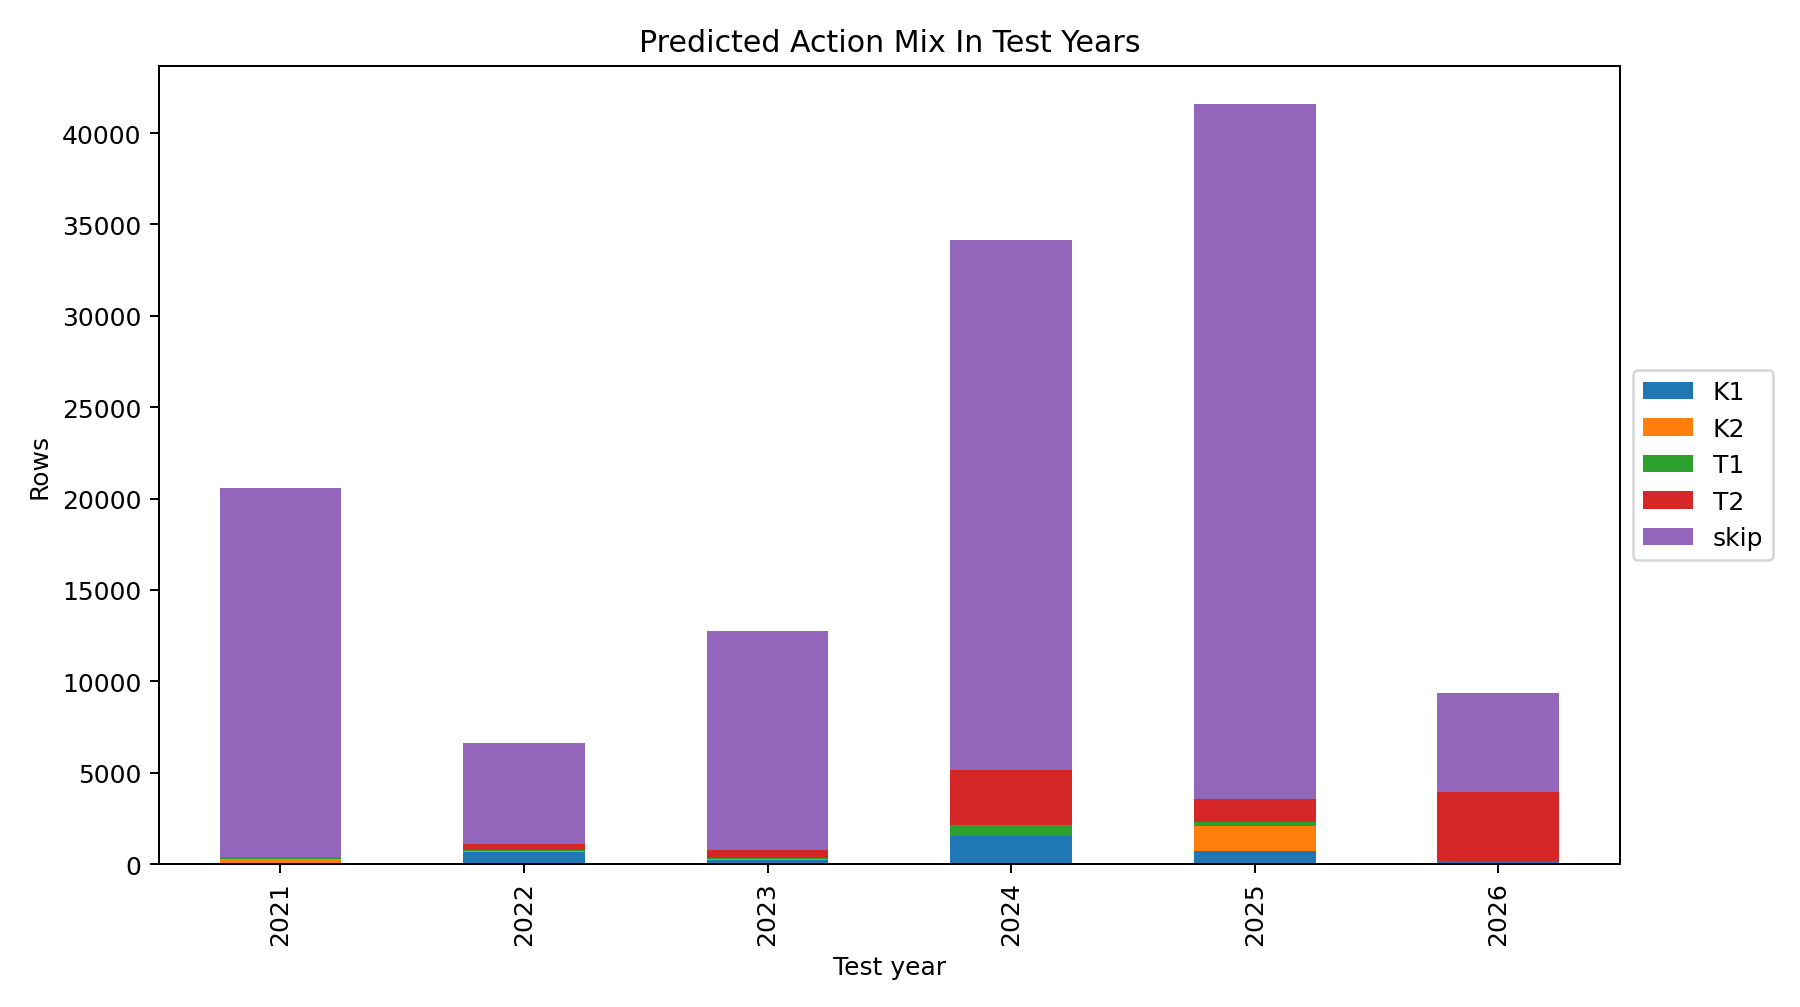
\includegraphics[width=0.92\linewidth]{figures/ml_lightgbm_action_mix.png}
  \caption{Predicted action mix by test year.}
  \label{fig:ml-action-mix}
\end{figure}



\begin{figure}[H]
  \centering
  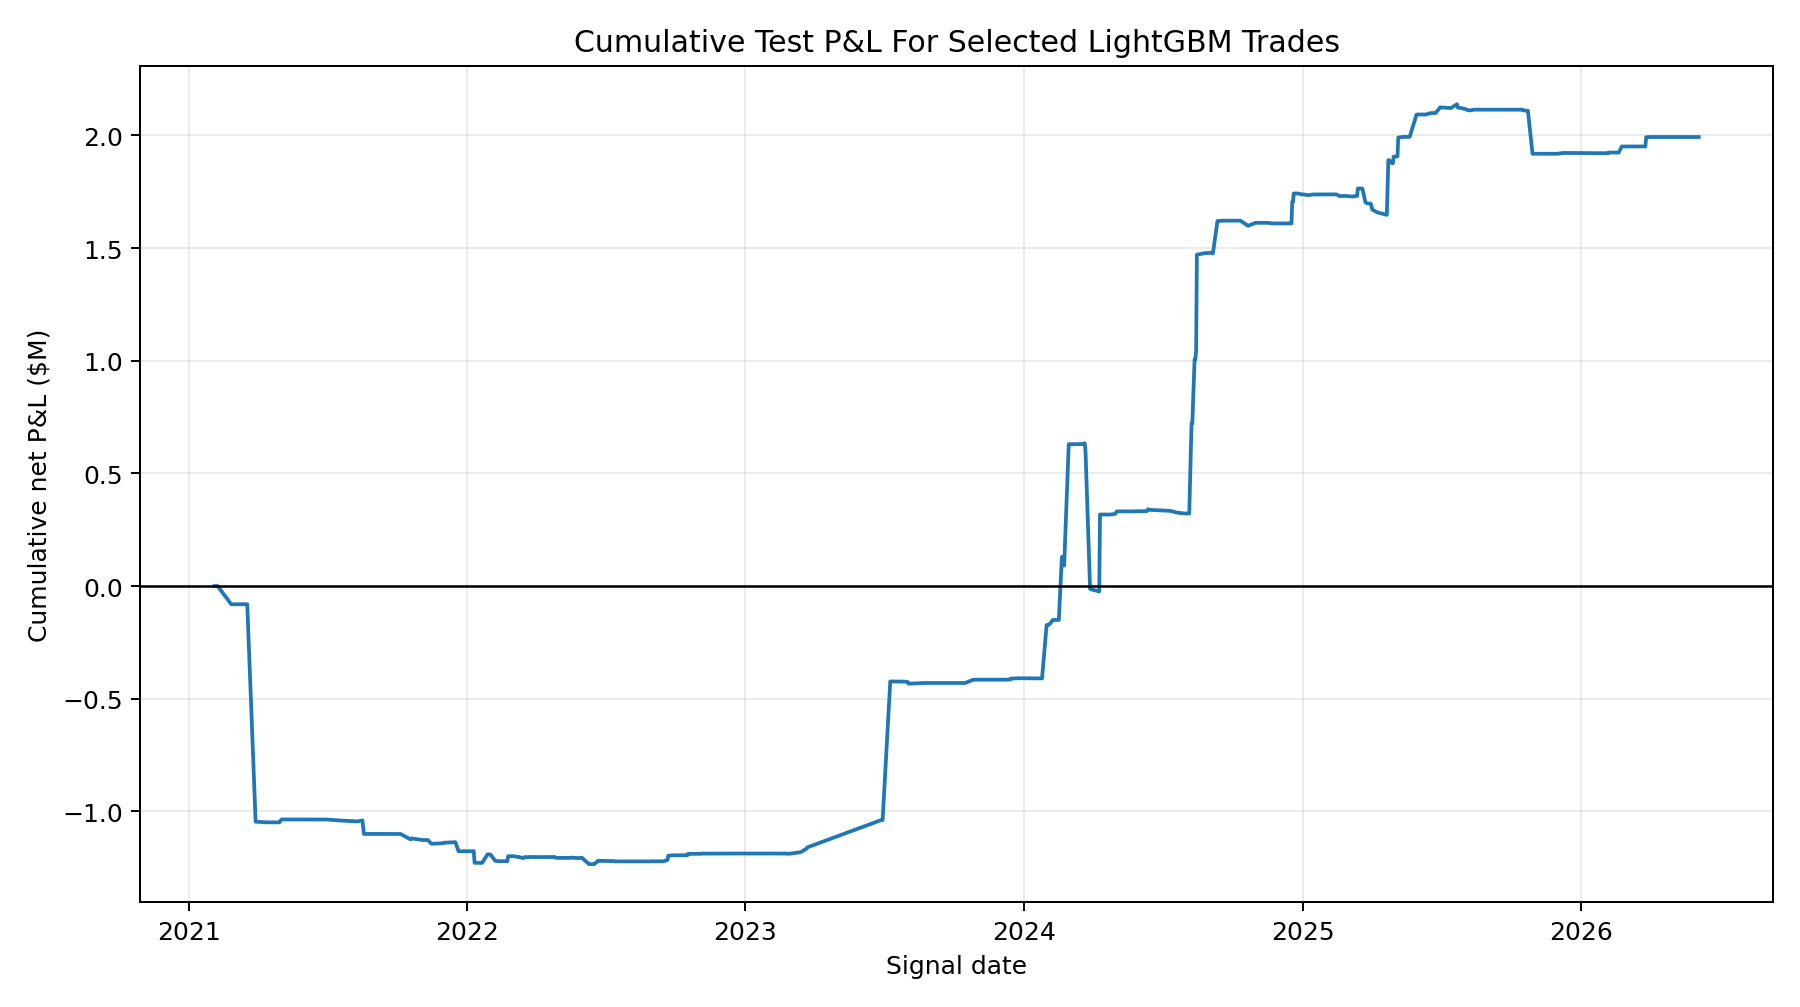
\includegraphics[width=0.92\linewidth]{figures/ml_lightgbm_cumulative_pnl.png}
  \caption{Cumulative out-of-sample test P\&L across selected LightGBM trades.}
  \label{fig:ml-cumulative-pnl}
\end{figure}


\section{Interpretation}

This first ML pass is useful but not yet publishable as a final model. It shows that the lifecycle
and signal-date features contain predictive information in several years, especially 2023--2026,
but performance is unstable in 2021 and near flat in 2022. That instability is important evidence:
the task is not solved by simply applying a classifier to all violations.

The strongest research direction is to improve decision quality rather than increase model size
immediately. Next steps should include expected-P\&L regression per action, capped P\&L targets,
probability calibration, lower invalid-selection penalties, and a Transformer over event days
\(-20\) through 0.

\section{Next Checks}

\begin{enumerate}
\item Add expected-P\&L LightGBM regressors for T1/T2/K1/K2 and compare against the current multiclass policy.
\item Penalize invalid exits directly in the target, not only in the report.
\item Report capped and winsorized P\&L to reduce concentration risk.
\item Add SHAP or feature importance after the model target is stable.
\end{enumerate}

\end{document}
